\documentclass[11pt]{article}

\usepackage[utf8]{inputenc}
\usepackage{amsmath}
\usepackage{amssymb}
\usepackage{parskip}
\usepackage{mathtools}
\usepackage{color}

\usepackage{graphicx}
\usepackage{caption}
\usepackage{enumitem}
%\usepackage{enumerate}
\usepackage{xcolor}
\usepackage{mdframed}
\usepackage{lipsum}
\usepackage{url}
\usepackage{subcaption}
\usepackage{MnSymbol,wasysym}
\usepackage{commentary-public}
\usepackage[noend,linesnumbered]{algorithm2e}
\usepackage{setspace} 
\DeclarePairedDelimiter\ceil{\lceil}{\rceil}
\DeclarePairedDelimiter\floor{\lfloor}{\rfloor}
\usepackage[left=1in,right=1in,top=1in,bottom=1in]{geometry}
\usepackage{amssymb}
%\usepackage{tabularx}
\usepackage{tabulary}

\let\oldemptyset\emptyset
\let\emptyset\varnothing

\begin{document}

\title{Polyglot Persistence : When One Size Does Not Fit All}
\author{Jules Testard}
\maketitle

\begin{abstract}
For a long time, SQL used to be the "one size fits all" solution, in the sense that any application could meet all of its requirements using only a SQL database. In the Big Data era, a number of new specialized system have emerged to meet the needs of the ever increasingly complex applications. Turing Award winner Michael Stonebreaker announced in 2006 that "the era of SQL had ended", in the sense that for any given application requirement there exists a number of new specialized system that can beat SQL to it; but there are applications whose requirements cannot be met by any single database. This led to the emergence of the so called "Polyglot Persistence" (PP) systems in which multiple specialized systems have to be used in coordination in order to meet all the requirements. Enabling such a coordination creates a number of challenges since specialized systems have been built to run independently and now have to be integrated together despite differing on a number of logical and architectural dimensions. In this paper, we present and discuss those challenges and analyze the current state of the art.
\end{abstract}

\section{Introduction}

%For a long time, relational database management systems (RDBMS) used to be the ?one size fits all? solution. From business data processing to analytics and data warehousing, any application could meet all of its requirements using only a SQL database. Since the early 2000's, the data 

% SQL once was the "one size for all" option
In the 1970's, the relational database management systems (RDBMS) were invented to solve the business transaction processing problem, in which data object needed to be stored and retrieved from disk efficiently for the first time. % System R citation
Between the 1970's and the 2000's, RDBMS have shown to become quite versatile and applicable to a number of number of other fields such as data warehousing, information retrieval... Such versatility made it convenient and appropriate to consider RDBMS a "one size fits all" solution, and build applications used a SQL database to handle all of its data management needs.

% SQL limitations
However, RDBMS do have their limitations. First, when the volume of data to be stored or the throughput of operation becomes too high, a system can either scale vertically (by getting a bigger machine) or horizontally (by getting more machines). A relational database doesn't scale well horizontally, and there is a limit of how big a single machine can become (bigger machine are quite expensive as well). Second, relational databases are restricted to a fixed schema which describes how the data is stored, and a change to the schema is difficult to perform, especially in an already running system. Finally, relational databases are based on the relational data and query model, and when the data and query model of an application becomes too different from the relational model, queries becomes too complex to express and too slow during execution.

% Specialized systems and their emergence.
In the early 2000's, the limitations of RBMS became more obvious as the number of applications grew exponentially. Stream processing required maintaining queries continuously despite a high insert rate, graph analysis and warehousing analytics required answering queries based on edges and columns respectively, rather than rows. Later in the mid-2000's, the volume and velocity of data for some applications became so high that horizontal scaling became a necessity and relational databases could not keep up with the performance requirements.
Likewise, the need for complex analytics over large amounts of data required the horizontal scalability and flexibility that only systems based on the Map Reduce ~\cite{Dean2008} paradigm could offer. As a result, specialized systems emerged for each of those fields and quite naturally outperformed RDBMS in their own field of specialization. Stonebreaker \& al, showed that even in the field of business transaction processing, the very problem were conceived for, RDBMS are outperformed by H-Store ~\cite{Stonebreaker2007}, a specialized system. The "one size fits all" paradigm requires RDBMS to perform decently under very different workload scenarios, making trade-offs when specialized systems need not make them. Figure ~\ref{fig:dblandscape} shows a recent landscape of specialized systems ~\cite{Aslett2012}.

\begin{figure}
 \centering
  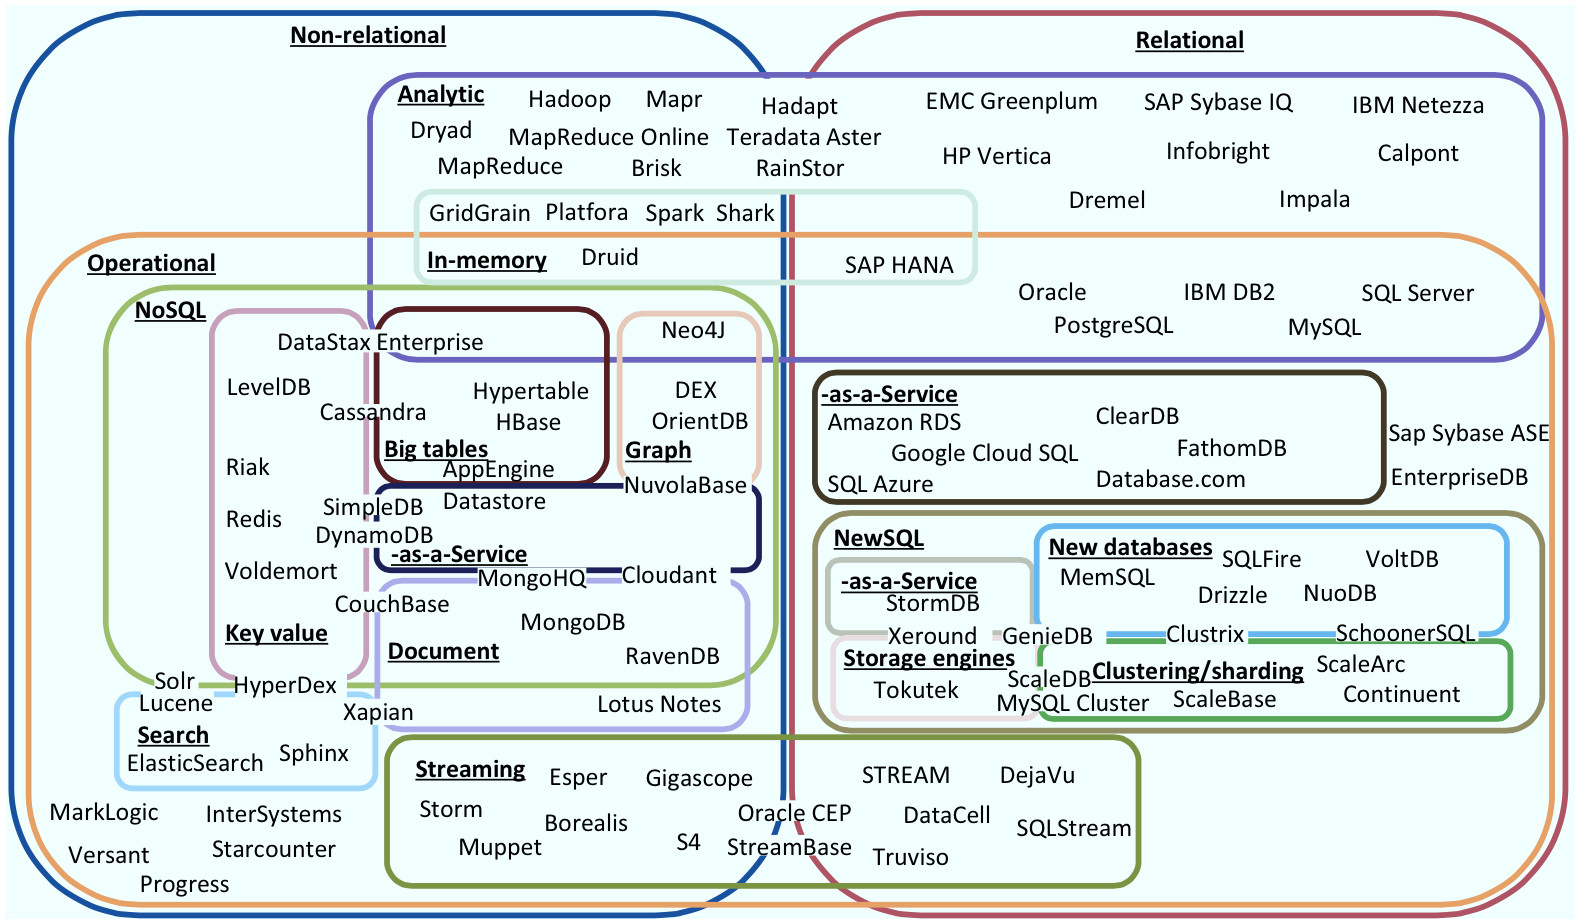
\includegraphics[width=0.8\textwidth]{images/DBLandscapeWithStream.png}
  \caption{Landscape of database systems available as of late 2012, many of which are very recent.}
  \label{fig:dblandscape}
\end{figure}

% Use an e-commerce running example.

%TODO : check that it is not a problem to reuse part of an article if we explicitly cite it. 
% Single System solution
The downside of having specialization is that naturally applications arise where an application's requirements aren't met by any single specialized system.Consider the situation of an e-commerce startup who just received the funding they required and wish to implement their data infrastructure. They come up with a list of features their application should provide : 

\begin{enumerate}[label=(\alph*)]
\item{The product manager has a very ambitious vision of what information customers can specify about themselves and other customers (preferences, ratings...) but isn't quite sure about the specifics, thus he expects the schema representing customers to vary significantly over the next few months. The products specifics are expected to vary significantly as well.}
\item{Like any other e-commerce website, customers can shop through the website using a shopping cart and finalize their purchase through a check out page. The shopping cart is transient and doesn't need to be stored after the purchase is finalized, but must always be quickly available. Customers can purchase items with store credits and the products managers are very careful about the integrity of the customer's store credit balance, thus want guarantees that its value will be immediately accurate after any finalized purchase, even if that means the customers has to wait a few milliseconds longer.}
\item{The entrepreneurs also imagine customers importing their friends from Facebook or other social networks, or make contacts on their own through the website. Such social information could then by used to provide recommendations to customers when they are browsing such as "your friends bought these accessories for this product".}
\item{Finally, the entrepreneurs want to understand better their clients. In the context of behavioral targeting, they wish to aggregate their user's unique clicks over the past hour, updated every 5 minutes. The number of clicks is expected to be very big, although loosing a few clicks isn't considered a big problem.}
\end{enumerate}

% TODO : Maybe think about putting this example later
%Another problem arises when changes in the application requirements mean the currently used storage system is not the best to handle the new requirements. If the application is tightly coupled to the storage system then changing storage systems would require substantial changes to the application codebase, which is something a developer would rather avoid.

No single database can satisfy all of these features. For example, feature 1 require customers and products data to be schema-less in order to adapt smoothly to application changes. Such a requirement would suggest using a document or key-value NoSQL store, but such a store wouldn't be able to satisfy the complex graph-based queries expected for feature 3.

Two approaches exist to solve this problem. The first option is to take an existing specialized system capable of doing $X$, and understand how to extend it to make it able to $Y$. Lim \& al ~\cite{Lim2013} provide three examples of such systems : i) \emph{MapReduce Online}, which adds pipelining and stream processing to the batch-oriented Map Reduce framework ~\cite{Condie2010}; ii) \emph{Online Aggregation for Map Reduce} which adds approximate answering capabilities to MapReduce ~\cite{Pansare2011}; HadoopDB, which enhances MapReduce's performance for SQL query processing while retaining MapReduce's fault-tolerance and fine-grained adaptivity ~\cite{Abouzeid2009}. This approach seems to consider going back to "one size fits all" systems, which begs the question how such systems will avoid the problems the RDBMS are confronted to.

\reminder{Jules : the above paragraph states a paragraph almost word for word from the Lim paper that we cite. Maybe should use less obvious paraphrasing instead?}

% Polyglot Persistence Requirements
In this paper, we take a different approach called "Polyglot Persistence" (PP) ~\cite{Fowler2012},  in which multiple specialized systems (called subsystems in this context) are used in coordination in order to meet all the requirements. This means the polyglot persistent system should achieve the following goals :

\begin{enumerate}[label=(\roman*)]
\item{\emph{Isolate the querying logic from the physical structure of the underlying storage systems} : if the query structure is dictated by the specificities of each storage subsystem then the complexity of the queries the user must write will increase. Worse, if any underlying storage system is replaced by another one (because of a change in application requirements, for example), the all the queries the application is using would have to be rewritten! Thus, such a system should provide a unique query interface with which the user can interact with any of the various subsystems using a common, unifying query language.}
\item{\emph{Making the best use of each subsystem}: this is the most important aspect of polyglot persistence systems. Specialized are better than RDBMS in their area of specialization, but are often worse in other types of interactions. For example, an RDBMS shouldn't be used to store the customer's information for our e-commerce startup since the customer schema is expected to vary significantly and relational databases are notoriously bad at dealing with schema changes. Each application requirement should be matched to the specialized system which handles it the best.}
\item{\emph{Maintaining consistency and integrity across subsystems} : when multiple data stores are being used together, then data must be partitioned between those stores, but those partitions are not necessarily logically independent. Data redundancy and integrity constraints may exists between the partitions: in our running example, if customers are stored in one database and orders in another, then adding an order to a non-existing customer should be prevented. Likewise, if the customers' address are stored with the orders, then changing a customer's address requires updating data in multiple data stores.}
\end{enumerate}

These goals come with a number of challenges provided below :

%Challenges
\begin{enumerate}
% TODO : warning, potential copyright infringement, reusing sentence from other paper.
\item{\emph{Choosing which systems to integrate given a set of requirements} : as seen on Figure ~\ref{fig:dblandscape}, the number of options is already large and growing larger every day. For a given application requirement, it isn't always clear which option is the best. Should the application developer use a SQL or NoSQL system? Within NoSQL, should she use a key-value store, a document database or column family system? How much more performance increase will a two-system solution provide over a one-system solution? How much more of a complexity overhead will a two system solution incur over a one system solution? As Lim \& al ~\cite{Lim2013}  point out, benchmarking storage options is not easy, in particular when application requirements are not quite set in stone yet.}
\item{\emph{Integrating multiple specialized system into a PP system} : once subsystems are chosen, they need to be integrated. Each specialized system was built independently and provides it's own query language (SQL, CQL, HiveQL, pig, N1QL, MongoDB...) and data model (relational, semi-structured, graph, key-value...). Yet a single query interface, common query language and common data model are required. The common query language and data model need to be as expressive as any of the query languages of the subsystems, in order to leverage fully the expressive power of every subsystem. }
\item{\emph{Optimizing queries in a PP system} :  in order to be relevant, a PP system needs to perform at least as well as any given single system solution. Optimization is particularly relevant in the context of queries targeting multiple subsystems, where the joining of data must be coordinated by the PP system. Depending on the architecture and design choices made for the subsystem integration, different kinds of optimization may be applied.}
\item{\emph{Updating the PP system while keeping it available and consistent} : updating data in any database systems poses the problem of consistency guarantees in the presence of multiple concurrent updates. The CAP theorem ~\cite{Gilbert2002} states that a distributed system can either be immediately consistent or always available, but not both. In the case of polyglot persistence, this means if an update to multiple subsystems has to be immediately consistent, then the PP system won't be available until all of the subsystems involved have been properly updated. Moreover, the subsystems themselves may have different consistency/availability tradeoffs which may have to be reconciled. How can we describe the availability and consistency characteristics of a PP system?}
\item{\emph{Deploying subsystems}: some specialized systems are meant to be deployed on clusters while others are meant to be deployed on individual machines. Should the developer of the PP system choose to deploy his subsystems on a common cluster which she owns or deploy each subsystem on a Platform-as-a-Service (PaaS) owned by a third party, or a mixture of both? Should she choose a common cluster, how can she allocate resources to individual subsystems? Some subsystems (especially those coming from the Hadoop ~\cite{Shvachko2010} ecosystem) separate their storage and compute components. Should the developer use the same storage component for multiple subsystems or use different storage components for each subsystem?}
\end{enumerate}

In this paper, we look at each of those challenges through our running example and survey existing solutions. Each challenge has its own section, and corresponding set of dimensions on which different solutions agree or differ. Some existing works tackle several of those challenges thus are mentioned once for each section in which they provide a solution. 

%\reminder{Jules : The introduction when considering context, running example, goals and challenges becomes really long. Should the challenges be split into another section?}


\section{Choosing the right specialized systems}

%As seen on Figure ~\ref{fig:dblandscape}, the number of options is already large and growing larger every day. For a given application requirement, it isn't always clear which option is the best. Should the application developer use a SQL or NoSQL system? Within NoSQL, should she use a key-value store, a document database or column family system? How much more performance increase will a two-system solution provide over a one-system solution? How much more of a complexity overhead will a two system solution incur over a one system solution? As Lim \& al ~\cite{Lim2013}  point out, benchmarking storage options is not easy, in particular when application requirements are not quite set in stone yet.

Relevant papers : ~\cite{Castrejon2013} ~\cite{Peidro2011} ~\cite{SNIA2012} ~\cite{Carlson2012} ~\cite{Truong2011}

\reminder{Jules : In this section, we show how to choose the right databases for the running example. This section will be updated later. However, for the purpose of having everything we need for the next section, we provide here the data stores which will be used by the running example : 
\begin{itemize}
\item{Products and Customers are to be stored on the document database MongoDB.}
\item{Orders are to be stored on the relational database MySQL.}
\item{The shopping cart is to be stored using the in-memory key-value store Redis.}
\item{The social network is to be stored on the graph database Neo4J.}
\item{The user activity logs are to be written to the column-oriented store HBase.}
\item{User activity monitoring is to be performed by Apache Storm.}
\end{itemize}
}

\section{Integrating specialized systems}

%Once subsystems are chosen, they need to be integrated. Each specialized system was built independently and provides it?s own query language (SQL, CQL, HiveQL, pig, N1QL, MongoDB...) and data model (relational, semi-structured, graph, key-value...). Yet a single query interface, common query language and common data model are required. The common query language and data model need to be as expressive as any of the query languages of the subsystems, in order to leverage fully the expressive power of every subsystem.

\subsection{Integrating data from multiple sources : historical review}

The goal of a PP system is to provide an unique query interface to interact with the various subsystems it provides. These subsystems each have their own The problem of integrating data coming from multiple sources is a classical problem in data integration which has been extensively studied ~\cite{Lenzerini2002}. 

Federated Query Processor MiddleWare Architecture

Most PP systems that have been studied focus on middle ware based architecture in which the user specifies a query which is then translated into sub components.

Each sub component corresponding to a fragment which is sent to individual subsystems.

These fragments are then translated into the subsystem's native query language and executed on those subsystems.

The results of the fragment queries are then returned to the middleware which joins them together to form a response to the user initial query.

This technique is inherited from the classical data integration integration problem that has been studied extensively in the 1990's.

Describe first what is the global as view approach 

\subsection{Finding a unifying data model and query language}

\subsubsection{procedural vs declarative approach}

Relevant papers : ~\cite{Lenzerini2002} ~\cite{Kirk1995} ~\cite{Katsis2009}
~\cite{Srivastava2006} ~\cite{Tatbul2010} ~\cite{Botan2009} ~\cite{Botan2010} ~\cite{Lim2013}
~\cite{Sharp2013} ~\cite{Cure2011} ~\cite{Atzeni2012} ~\cite{Sellami2014} ~\cite{Sellami2013}
~\cite{Ong2014} ~\cite{Ong2015} ~\cite{Boag2010} ~\cite{Ives2002} ~\cite{Borkar2006}
~\cite{Liu2010} ~\cite{Fowler2012}

 \reminder{Jules : In this section, we show what the generic, classical middleware query architecture looks like with the databases chosen above.}
 
 
\begin{figure}
 \centering
  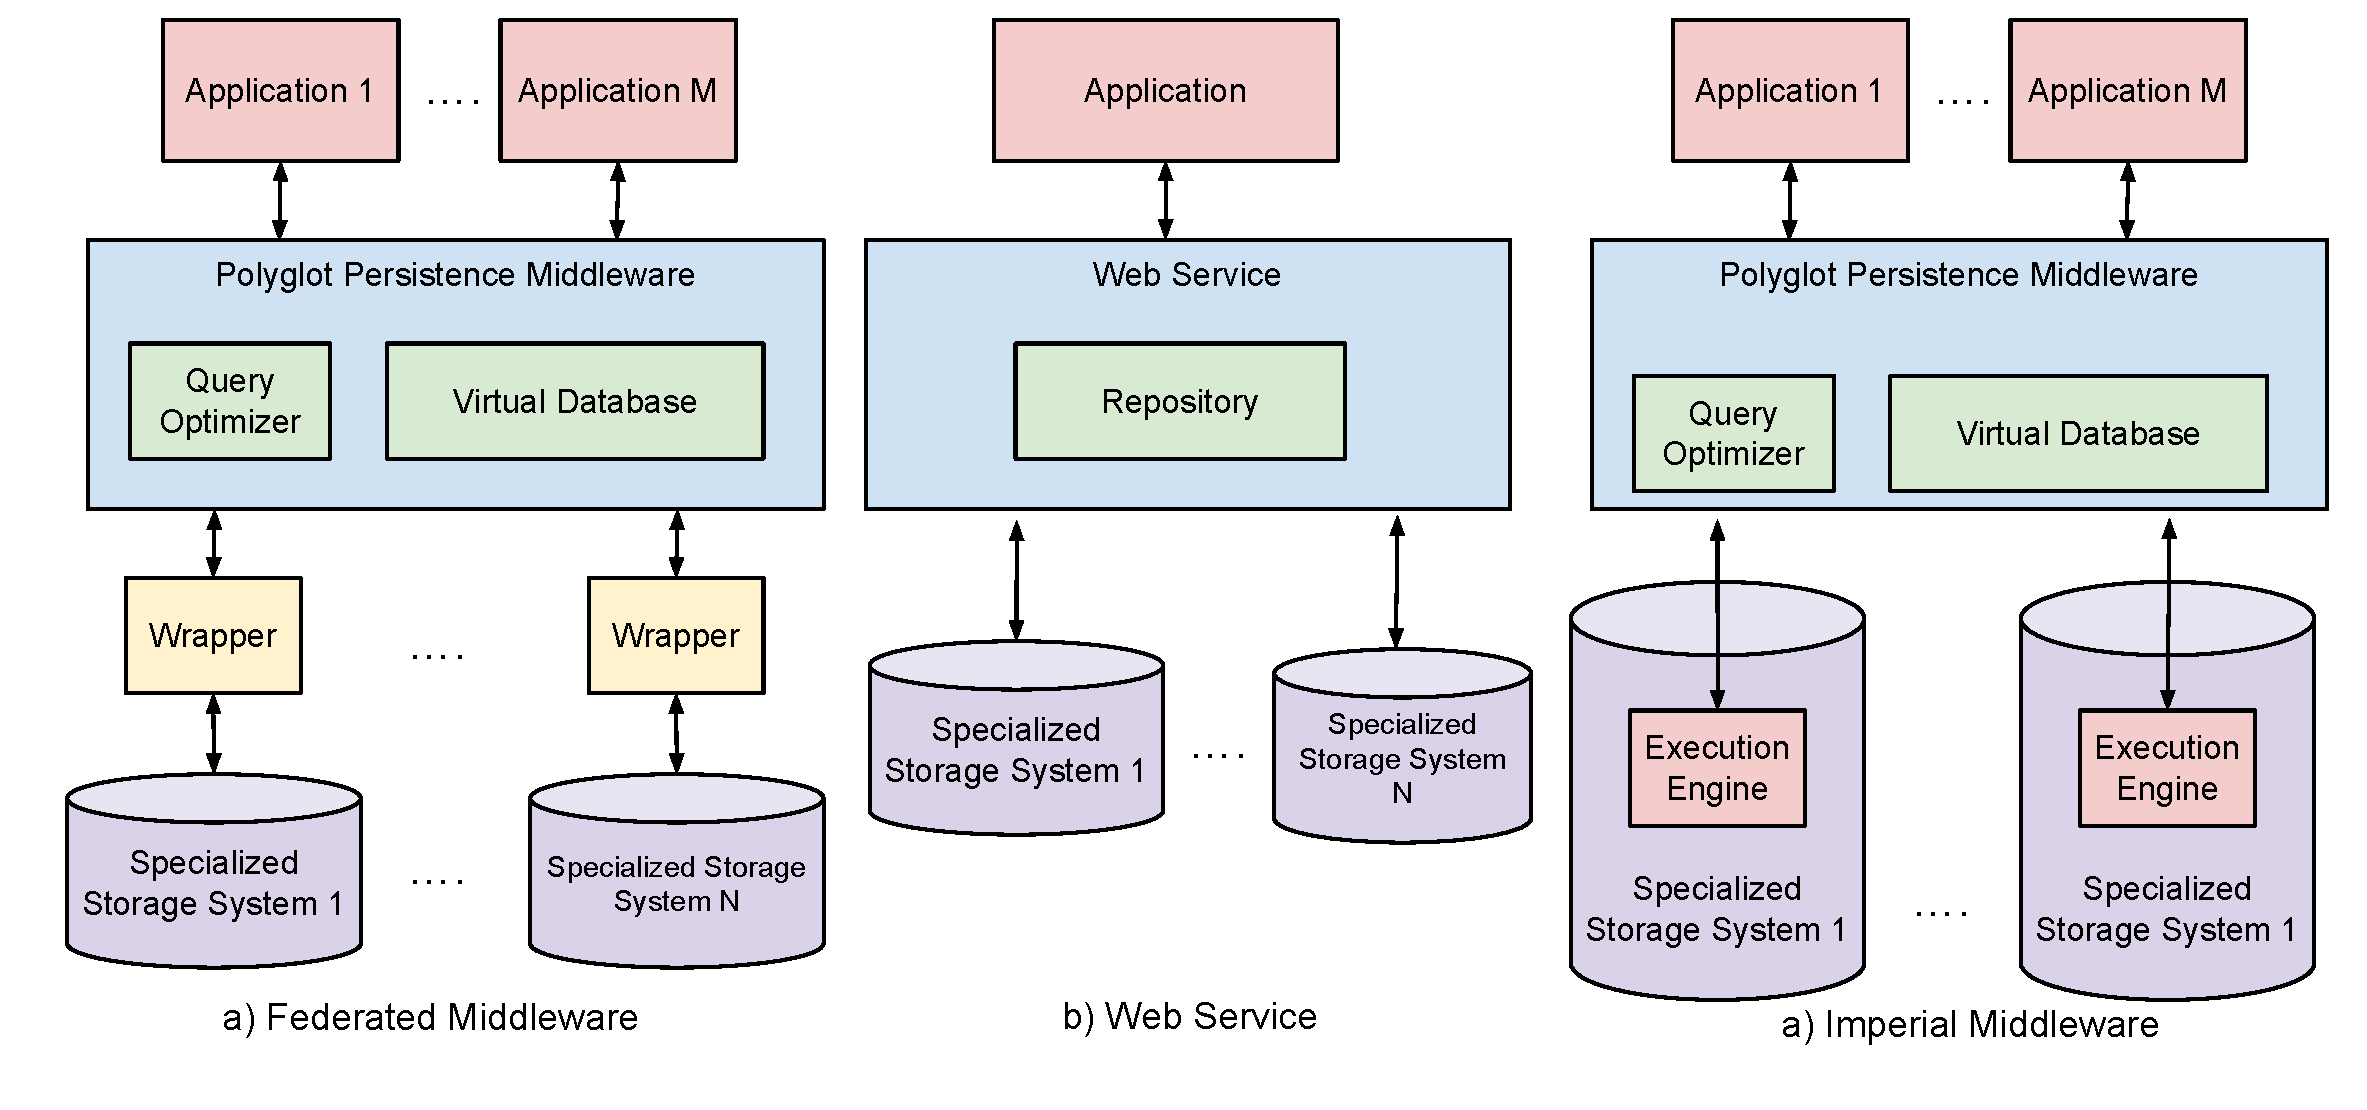
\includegraphics[width=0.8\textwidth]{images/MiddlewareArchitecture.pdf}
  \caption{Classical Middleware Data Integration Architecture applied to our running example}
  \label{fig:dblandscape}
\end{figure}





\section{Optimizing queries in a PP system}

%In order to be relevant, a PP system needs to perform at least as well as any given single system solution. Optimization is particularly relevant in the context of queries targeting multiple subsystems, where the joining of data must be coordinated by the PP system. Depending on the architecture and design choices made for the subsystem integration, different kinds of optimization may be applied.

Relevant Papers : ~\cite{bugiotti2015} ~\cite{LeFevre2014}  ~\cite{Haas1997} ~\cite{Srivastava2006} ~\cite{Halevy2001}
 ~\cite{Botan2009} ~\cite{Botan2010} ~\cite{Lim2013} ~\cite{Cure2011} ~\cite{Papakonstantinou1998}  ~\cite{Ives2002}  ~\cite{Borkar2006}
  ~\cite{Liu2010}

 
 % Database optimization, database hot-Swapping : choose which database to use for query computation as part of the query plan.

\section{Updating the PP system while keeping it available and consistent}

%Updating data in any database systems poses the problem of consistency guarantees in the presence of multiple concurrent updates. The CAP theorem ~\cite{Gilbert2002} states that a distributed system can either be immediately consistent or always available, but not both. In the case of polyglot persistence, this means if an update to multiple subsystems has to be immediately consistent, then the PP system won't be available until all of the subsystems involved have been properly updated. Moreover, the subsystems themselves may have different consistency/availability tradeoffs which may have to be reconciled. How can we describe the availability and consistency characteristics of a PP system?

Relevant Papers :  ~\cite{Botan2009} ~\cite{Botan2010} ~\cite{Sharp2013}  ~\cite{Atzeni2012} ~\cite{Sellami2014} ~\cite{Sellami2013}
 ~\cite{Fowler2012} ~\cite{Das2013}

\section{Deploying subsystems}

%Some specialized systems are meant to be deployed on clusters while others are meant to be deployed on individual machines. Should the developer of the PP system choose to deploy his subsystems on a common cluster which she owns or deploy each subsystem on a Platform-as-a-Service (PaaS) owned by a third party, or a mixture of both? Should she choose a common cluster, how can she allocate resources to individual subsystems? Some subsystems (especially those coming from the Hadoop ~\cite{Shvachko2010} ecosystem) separate their storage and compute components. Should the developer use the same storage component for multiple subsystems or use different storage components for each subsystem?

Relevant Papers : ~\cite{bugiotti2015} ~\cite{LeFevre2014} ~\cite{Lim2013}  ~\cite{Sellami2013}

%\section{Synthesis}

\bibliography{bibliography}{}
\bibliographystyle{plain}

\end{document}







